\documentclass{beamer}

\usepackage[utf8]{inputenc}
\usepackage[T1]{fontenc}

\usepackage[english]{babel}
\usepackage{amsmath}
\usepackage{cleveref}
\usepackage{amssymb}
\usepackage{mathtools}

%%Numbers, expectation
\newcommand{\N}{\mathbb{N}}
\newcommand{\E}{\mathbb{E}}
\renewcommand{\P}{\mathbb{P}}
\newcommand{\Var}{\mathbb{V}}
\newcommand{\R}{\mathbb{R}}
\newcommand{\D}{\mathcal{D}}
\newcommand{\B}{\mathcal{B}}
\newcommand{\Dh}{\D_h}
\renewcommand{\phi}{\varphi}
\newcommand*\diff{\mathop{}\!\mathrm{d}} % integral

%% mathoperator
\DeclareMathOperator*{\argmax}{arg\,max}
\DeclareMathOperator*{\argmin}{arg\,min}
\DeclareMathOperator*{\dom}{dom}
\DeclareMathOperator*{\sign}{sign}
\DeclareMathOperator*{\diag}{diag}

\DeclareMathOperator*{\Cov}{Cov}
\DeclareMathOperator*{\Cor}{Corr}
\DeclareMathOperator*{\Id}{Id}

%proximal operator
\newcommand{\prox}[3][]{\operatorname{prox}^{#1}_{#2}\left(#3 \right)}

\usepackage{xcolor}

%% sort citations by increasing number
\usepackage[sort,nocompress]{cite}

\usepackage{graphicx}% http://ctan.org/pkg/graphicx
\graphicspath{{../figures/}{../../figures}{../../memes}} %Setting the graphicspath
\usepackage{caption,subcaption}

\usepackage{tikz}
\usepackage{pgfplots}
\usetikzlibrary{backgrounds}
\usetikzlibrary{intersections}
\usepgfplotslibrary{fillbetween}

% \usepackage[right]{showlabels}


%%
\theoremstyle{plain}
\newtheorem{prop}{Proposition}[section]
\newtheorem{algo}{Algorithm}[section]
\newtheorem{assumption}{Assumption}
\theoremstyle{remark}
\newtheorem{remark}{Remark}[section]

% cref
\crefname{assumption}{Assumption}{Assumptions}
\crefname{equation}{}{}

\usepackage{autonum}

\usepackage{bm} %% bold math symbols

\usepackage{bbm} %% for \mathbbm{1}


% algorithmic environment
\usepackage{algorithm}
\usepackage[noend]{algpseudocode}

% for some reason this was required on one void linux installation (but not the other)
\usepackage{sansmathaccent}
\pdfmapfile{+sansmathaccent.map}

\author{Axel Böhm}

% shows which section we're in
\usetheme{Darmstadt}

% page number
\setbeamertemplate{footline}[frame number]
\setbeamercolor{page number in head/foot}{fg=gray}


% display things like onslide or visible already before but grayed out
\setbeamercovered{transparent}

% set the itemize item symbol as a diamond
\setbeamertemplate{itemize item}{$\diamond$}
% set the itemize subitem symbol as a triangle
\setbeamertemplate{itemize subitem}{$\blacktriangleright$}

% set the enumerate item symbol as a roman numbers
\setbeamertemplate{enumerate item}{(\roman{enumi})}


% https://openai.com/blog/deep-double-descent/

\title{Subgradient method}
\date{\today}

\begin{document}
\maketitle
\frame{\tableofcontents[currentsection]}

\section{Introduction}%

\begin{frame}
  \frametitle{Smooth vs. nonsmooth}

  \begin{equation}
    \min_x \, f(x)
  \end{equation}

  \begin{block}{$f$ is \emph{smooth} and convex}
    Smoothness means $\Vert \nabla f(x) - \nabla f(y) \Vert \le L \Vert x-y \Vert$:
    \begin{equation}
      \begin{aligned}
        \text{GD:} \quad x_{k+1} = x_k - \alpha_k \nabla f(x_k) \\
        f(x_k) - f^* = \mathcal{O}(\frac{1}{k})
      \end{aligned}
    \end{equation}
    if the stepsize fulfills $\alpha_k \le 1/L$.
  \end{block}
  \begin{block}{nonsmooth but convex: \textbf{subgradient method}}
    \begin{equation}
      \begin{aligned}
        \left\lfloor \begin{array}{l}
                 \text{pick $g_k \in \partial f(x_k)$}
                 x_{k+1} = x_k - \alpha_k g_k \\
               \end{array}\right.
        f(x_k) - f^* = \mathcal{O}(\frac{1}{\sqrt{k}})
      \end{aligned}
    \end{equation}
  \end{block}
\end{frame}

\section{convergence}%
\label{sec:}
\begin{frame}
  \frametitle{Convergence statement}
  \begin{theorem}
    $f$ is convex, subgradients are bounded $\Vert g(x) \Vert \le G$ for all $g(x)\in \partial f(x)$. Then,
    \begin{equation}
      f(\bar{x}_k) - f^* \le \frac{\Vert x_1-x^*\Vert^2 + G^2 \sum_{i=1}^{k}\alpha_i^2}{2 \sum_{i=1}^{k}\alpha_i}
    \end{equation}
    for the averaged iterates $\bar{x}_k = \frac{\sum_{i=1}^{k} \alpha_i x_i }{\sum_{i=1}^{k} \alpha_i}$
  \end{theorem}
\end{frame}

\begin{frame}
  \frametitle{Proof}
  \vspace{-0.5cm}
  \begin{equation}
    \begin{aligned}
      \Vert x_{k+1} - x^* \Vert^2 &\le \Vert x_k - \alpha_k g_k - x^* \Vert^2 \\
      &= \Vert x_k-x^* \Vert^2 + 2 \alpha_k \langle g_k, x^*-x_k \rangle + \alpha^2 \Vert g_k \Vert^2.
    \end{aligned}
  \end{equation}
  Using the subgradient ineq. $\langle g_k , x^* -x_k \rangle \le f(x^*) - f(x_k)$
  % \begin{equation}
  %   \langle g_k , x^* -x_k \rangle \le f(x^*) - f(x_k)
  % \end{equation}
  we deduce
  \begin{equation}
    \Vert x_{k+1} - x^* \Vert^2 \le \Vert x_k-x^* \Vert^2 + 2 \alpha_k(f(x^*) - f(x_k)) + \alpha_k^2 \Vert g_k \Vert^2.
  \end{equation}
  Via the \emph{bounded subgradient} assumption
  \begin{equation}
    2\sum_{i=1}^{k}  \alpha_i(f(x_i) - f(x^*)) + \Vert x_{k+1} - x^* \Vert^2 \le \Vert x_1-x^* \Vert^2 +  \sum_{i=1}^{k} \alpha_i^2 G^2.
  \end{equation}
  Using Jensens inequality % give intuition for 2-d case
  \begin{equation}
    \sum_{i} \lambda_i f(x_i) \ge \sum_{i} f \left( \frac{\sum_{i} \lambda_i x_i}{\sum_{i}\lambda_i} \right)
  \end{equation}
  we obtain
  \begin{equation}
    2\sum_{i=1}^{k}  (f(\bar{x}_k) - f(x^*)) + \Vert x_{k+1} - x^* \Vert^2 \le \Vert x_1-x^* \Vert^2 +  \sum_{i=1}^{k} \alpha_i^2 G^2.
  \end{equation}

\end{frame}


\begin{frame}
  \frametitle{How to choose the stepsize?}
  \begin{equation}
    f(\bar{x}_k) - f^* \le \frac{\Vert x_1-x^*\Vert^2 + G^2 \sum_{i=1}^{k}\alpha_i^2}{2 \sum_{i=1}^{k}\alpha_i}
  \end{equation}
  Clearly $\alpha_i = \ell_2\ \ell_1$ leads convergence, for example $1/i$.
  However, $\alpha_i = \mathcal{O}(1/\sqrt{i})$ gives
  \begin{equation}
    \sum \alpha_i = (\frac{1}{\sqrt{1}} + \frac{1}{\sqrt{2}} + \cdots +  \frac{1}{\sqrt{k}}) > \sqrt{k}\\
    \sum \alpha_i^2 = (\frac{1}{1} + \frac{1}{2} + \cdots + \frac{1}{k}) \approx \log(k)
  \end{equation}

  \begin{equation}
    f(\bar{x}_k) - f^* \le \frac{\Vert x_1-x^*\Vert^2 + G^2 \log(k)}{2 \sqrt{k}}
  \end{equation}
  gives complexity
  \begin{equation}
    \mathcal{O}\left(\frac{\log(k)}{k}\right) =: \tilde{\mathcal{O}}\left(\frac{1}{k}\right)
  \end{equation}

\end{frame}


\begin{frame}
  \frametitle{Projected subgradient method}
  \begin{equation}
    \text{(constrained setting)} \quad \min_{x\inC}\, f(x)
  \end{equation}
  \begin{equation}
    x_{k+1} = P_C( x_k- \alpha_k g_k )
  \end{equation}
  By using the fact that the projection is a contraction
  \begin{equation}
    \Vert P_C(x) - P_C(y) \Vert \le \Vert x-y \Vert
  \end{equation}
  we can deduce the exact same inequality as before
  \begin{equation}
      \Vert x_{k+1} - x^* \Vert^2 &= \Vert P_C(x_k - \alpha_k g_k) - x^* \Vert^2 \\
      &\le \Vert x_k - \alpha_k g_k - x^* \Vert^2 \\
      &= \Vert x_k-x^* \Vert^2 + 2 \alpha_k \langle g_k, x^*-x_k \rangle + \alpha^2 \Vert g_k \Vert^2\\
      &\le \Vert x_k-x^* \Vert^2 + 2 \alpha_k (f^* - f(x_k))+ \alpha^2 \Vert g_k \Vert^2.
  \end{equation}
\end{frame}



\begin{frame}
  \frametitle{If $C$ is bounded we can improve a bit}

\end{frame}


\begin{frame}
  \frametitle{Polyak stepsize}
  Let's revisit the convergence proof of the subgradient method
  \begin{equation}
    \begin{aligned}
      \Vert x_{k+1} - x^* \Vert^2 &\le \Vert x_k - \alpha_k g_k - x^* \Vert^2 \\
      &= \Vert x_k-x^* \Vert^2 + 2 \alpha_k \langle g_k, x^*-x_k \rangle + \alpha^2 \Vert g_k \Vert^2\\
      &\le \Vert x_k-x^* \Vert^2 + 2 \alpha_k (f^* - f(x_k))+ \alpha^2 \Vert g_k \Vert^2.
    \end{aligned}
  \end{equation}
  Can we pick $\alpha_k$ such that the RHS is minimized?
  \begin{equation}
    \min_\alpha \, \alpha^2 \Vert g_k \Vert^2 + 2 \alpha_k (f^* - f(x_k))
  \end{equation}
  gives
  \begin{equation}
    \alpha^* = \frac{f(x_k)-f^*}{\Vert g_k \Vert^2}
  \end{equation}
  \begin{equation}
      \Vert x_{k+1} - x^* \Vert^2 = \Vert x_k-x^* \Vert^2 - {\left( \frac{f(x_k)-f^*}{\Vert g_k \Vert} \right)}^2
  \end{equation}
\end{frame}

\begin{frame}
  \frametitle{Poljak stepsize [contd]}
  \textit{}
  \begin{itemize}
    \item Requires us to know the optimal objective function value
    \item can be the case in certain setting:
          separable data, feasibility problems
    \item modern deep learning interpolation setting
  \end{itemize}

  \onslide<2->{%
    \begin{figure}[ht]
      \centering
      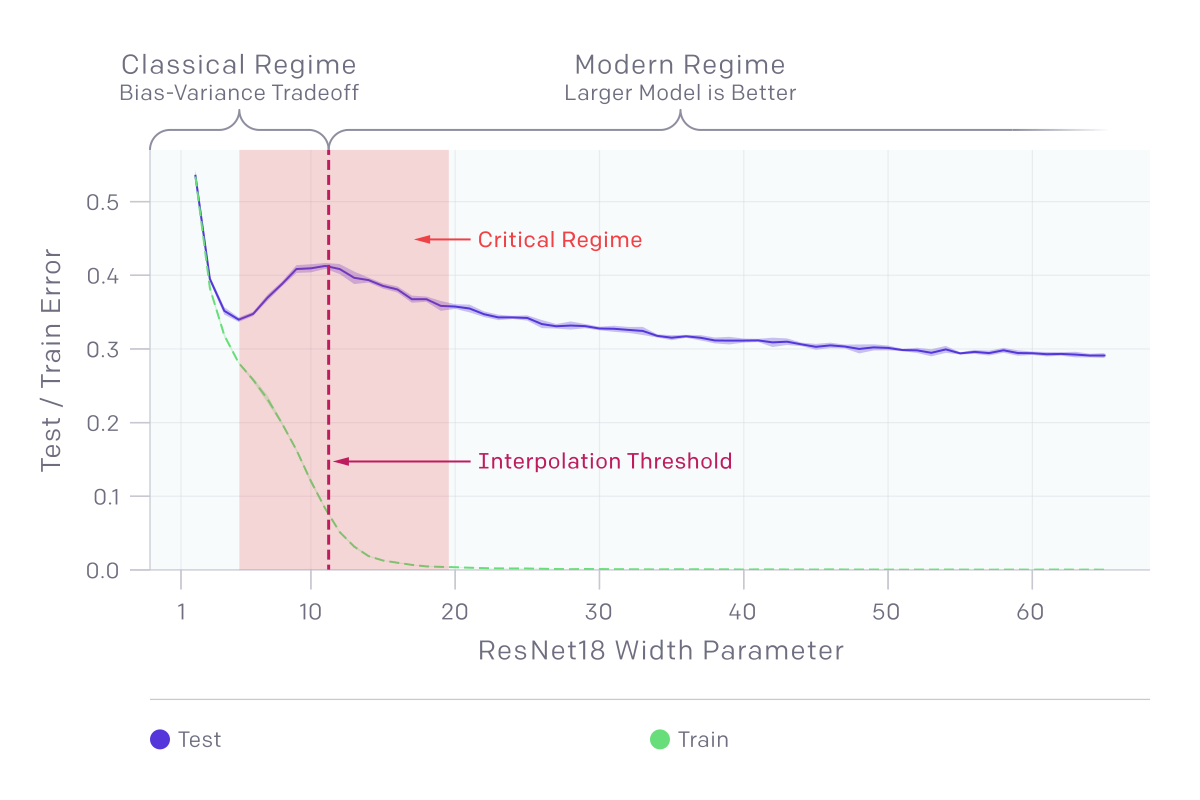
\includegraphics[\width=0.5\textwidth]{modern-regime.svg}
      \caption{Interpolation / overparametrization regime}
    \end{figure}
  }

\end{frame}


\end{document}
